\begin{figure}
  \centering

  \small

  \newcommand{\w}[1]{\textcolor{white}{#1}}
  \def\svgwidth{0.9\textwidth}

  % INKSCAPE
%% Creator: Inkscape inkscape 0.91, www.inkscape.org
%% PDF/EPS/PS + LaTeX output extension by Johan Engelen, 2010
%% Accompanies image file 'vope_all_higher_mean.eps' (pdf, eps, ps)
%%
%% To include the image in your LaTeX document, write
%%   \input{<filename>.pdf_tex}
%%  instead of
%%   \includegraphics{<filename>.pdf}
%% To scale the image, write
%%   \def\svgwidth{<desired width>}
%%   \input{<filename>.pdf_tex}
%%  instead of
%%   \includegraphics[width=<desired width>]{<filename>.pdf}
%%
%% Images with a different path to the parent latex file can
%% be accessed with the `import' package (which may need to be
%% installed) using
%%   \usepackage{import}
%% in the preamble, and then including the image with
%%   \import{<path to file>}{<filename>.pdf_tex}
%% Alternatively, one can specify
%%   \graphicspath{{<path to file>/}}
%% 
%% For more information, please see info/svg-inkscape on CTAN:
%%   http://tug.ctan.org/tex-archive/info/svg-inkscape
%%
\begingroup%
  \makeatletter%
  \providecommand\color[2][]{%
    \errmessage{(Inkscape) Color is used for the text in Inkscape, but the package 'color.sty' is not loaded}%
    \renewcommand\color[2][]{}%
  }%
  \providecommand\transparent[1]{%
    \errmessage{(Inkscape) Transparency is used (non-zero) for the text in Inkscape, but the package 'transparent.sty' is not loaded}%
    \renewcommand\transparent[1]{}%
  }%
  \providecommand\rotatebox[2]{#2}%
  \ifx\svgwidth\undefined%
    \setlength{\unitlength}{842.296bp}%
    \ifx\svgscale\undefined%
      \relax%
    \else%
      \setlength{\unitlength}{\unitlength * \real{\svgscale}}%
    \fi%
  \else%
    \setlength{\unitlength}{\svgwidth}%
  \fi%
  \global\let\svgwidth\undefined%
  \global\let\svgscale\undefined%
  \makeatother%
  \begin{picture}(1,0.70675867)%
    \put(0,0){\includegraphics[width=\unitlength]{vope_all_higher_mean.eps}}%
    \put(0.19549212,0.32835986){\color[rgb]{1,1,1}\makebox(0,0)[b]{\smash{}}}%
    \put(0.11659136,0.27897104){\color[rgb]{0,0,0}\makebox(0,0)[b]{\smash{$\mu_i$}}}%
    \put(0.80742572,0.27897104){\color[rgb]{0,0,0}\makebox(0,0)[b]{\smash{$\mu_{i+1}$}}}%
    \put(0.11611712,0.54517651){\color[rgb]{0,0,0}\makebox(0,0)[b]{\smash{\w{$\pi_i$}}}}%
    \put(0.0957776,0.0813595){\color[rgb]{0,0,0}\makebox(0,0)[b]{\smash{}}}%
    \put(0.2327737,0.38332379){\color[rgb]{1,1,1}\makebox(0,0)[b]{\smash{\w{$\delta_i$}}}}%
    \put(0.92388196,0.38358593){\color[rgb]{1,1,1}\makebox(0,0)[b]{\smash{\w{$\delta_{i+1}$}}}}%
    \put(0.23523854,0.03888422){\color[rgb]{0,0,0}\makebox(0,0)[b]{\smash{$\hat{\mu}_i$}}}%
    \put(0.92230053,0.03888422){\color[rgb]{0,0,0}\makebox(0,0)[b]{\smash{$\hat{\mu}_{i+1}$}}}%
    \put(0.23472904,0.54441348){\color[rgb]{0,0,0}\makebox(0,0)[b]{\smash{\w{$\hat{\pi}_i$}}}}%
    \put(0.80681477,0.06924476){\color[rgb]{0,0,0}\makebox(0,0)[b]{\smash{$\mu_{i+1}$}}}%
    \put(0.23268947,0.27996019){\color[rgb]{1,1,1}\makebox(0,0)[b]{\smash{\w{$\varepsilon_i$}}}}%
    \put(0.92379785,0.28022233){\color[rgb]{1,1,1}\makebox(0,0)[b]{\smash{\w{$\varepsilon_{i+1}$}}}}%
    \put(0.23724135,0.62279812){\color[rgb]{0,0,0}\makebox(0,0)[b]{\smash{\footnotesize \w{$p_{i1}$}}}}%
    \put(0.17471894,0.58543147){\color[rgb]{0,0,0}\makebox(0,0)[b]{\smash{\tiny \w{$1$}}}}%
    \put(0.3345943,0.54705278){\color[rgb]{0,0,0}\makebox(0,0)[b]{\smash{\footnotesize \w{$p_{i2}$}}}}%
    \put(0.01194257,0.66674898){\color[rgb]{0,0,0}\makebox(0,0)[lb]{\smash{1}}}%
    \put(0.01160093,0.54411984){\color[rgb]{0,0,0}\makebox(0,0)[lb]{\smash{2}}}%
    \put(0.00653804,0.44819157){\color[rgb]{0,0,0}\makebox(0,0)[lb]{\smash{3\textsf{A}}}}%
    \put(0.00653845,0.28672814){\color[rgb]{0,0,0}\makebox(0,0)[lb]{\smash{3\textsf{B}}}}%
    \put(0.0113686,0.18795052){\color[rgb]{0,0,0}\makebox(0,0)[lb]{\smash{4}}}%
    \put(0.00651485,0.13476256){\color[rgb]{0,0,0}\makebox(0,0)[lb]{\smash{5\textsf{A}}}}%
    \put(0.00651485,0.07872525){\color[rgb]{0,0,0}\makebox(0,0)[lb]{\smash{5\textsf{B}}}}%
    \put(0.01169903,0.02743687){\color[rgb]{0,0,0}\makebox(0,0)[lb]{\smash{6}}}%
    \put(0.80644179,0.54529522){\color[rgb]{0,0,0}\makebox(0,0)[b]{\smash{\w{$\pi_{i+1}$}}}}%
    \put(0.92505377,0.54453219){\color[rgb]{0,0,0}\makebox(0,0)[b]{\smash{\w{$\hat{\pi}_{i+1}$}}}}%
    \put(0.35439399,0.50223398){\color[rgb]{0,0,0}\makebox(0,0)[b]{\smash{\tiny \w{$1$}}}}%
    \put(0.68070956,0.48008157){\color[rgb]{0,0.48235294,0.61568627}\makebox(0,0)[lb]{\smash{\footnotesize $\alpha_{i,i+1}^2$}}}%
    \put(0.52457087,0.61575879){\color[rgb]{0.62352941,0,0.52941176}\makebox(0,0)[lb]{\smash{\footnotesize $\alpha_{i,i+1}^2$}}}%
    \put(0.32634829,0.47686284){\color[rgb]{0.62352941,0,0.52941176}\makebox(0,0)[lb]{\smash{\footnotesize $\exp(\omega_i)$}}}%
    \put(0.2908826,0.48270342){\color[rgb]{0,0,0}\makebox(0,0)[b]{\smash{\w{$\nu_i$}}}}%
    \put(0.58127124,0.03868044){\color[rgb]{0,0.78431373,1}\makebox(0,0)[b]{\smash{\footnotesize $\alpha_{i,i+1}$}}}%
    \put(0.12062558,0.0698889){\color[rgb]{0,0,0}\makebox(0,0)[b]{\smash{$\mu_i$}}}%
  \end{picture}%
\endgroup%

  \caption{Zoomed-in version of the coupling between a hierarchical level $i$ with its parent $i+1$ in the case of \textsf{VAPE} coupling: implementing the differential equations that describe within-trial dynamics of the nodes.}
  \label{\figlabel}
\end{figure}
